<<<<<<< HEAD
%Joint Math Meetings, January 16, 2014
\documentclass[10pt,compress]{beamer} %slides and notes
\usepackage{amsmath,datetime,xmpmulti,mathtools,bbm,array,booktabs,alltt,xspace,mathabx,tikz,pifont,graphicx}
%\usepackage[autolinebreaks]{mcodefred}
\usepackage[author-year]{amsrefs}
\usetikzlibrary{arrows}
\usetheme{FredIIT}

\setlength{\parskip}{2ex}
\setlength{\arraycolsep}{0.5ex}

%\logo{\includegraphics[width=0.5cm]{IIT_mark_1c_red.eps}}
\logo{\includegraphics[width=0.5cm]{MengerIITRedGray.pdf}}

\title[Error Estimation for Sobol' Cubature]{Reliable Error Estimation for Cubature Using \\ Sobol' Sequences}
\author[hickernell@iit.edu]{Fred J. Hickernell}
\institute{\small{Department of Applied Mathematics,  Illinois Institute of Technology \\
\url{hickernell@iit.edu} \quad
\url{www.iit.edu/~hickernell}\\[2ex]
Joint work with Llu\'is Antoni Jim\'enez Rugama}\\[2ex]
Supported by NSF-DMS-1115392}
\date[MCQMC 2014]{April 10, 2014}

%The error in approximating the multidimensional integral $\int_{[0,1)^d} f(\boldsymbol{x}) \, {\rm d} \boldsymbol{x}$ by the sample average $n^{-1} \sum_{i=0}^{n-1} f(\boldsymbol{x}_i)$ depends on both the sampling scheme, $\{\boldsymbol{x}_0, \boldsymbol{x}_1, \ldots \}$, and the integrand, $f$.  Quasi-Monte Carlo methods, such as Sobol' sampling, are often substantially more efficient than IID sampling for evaluating multidimensional integrals.  A reliable data-based error bound is needed so that one can automatically determine the appropriate sample size, $n$, to satisfy a user-supplied error tolerance $\varepsilon$.  Koksma-Hlawka error bounds require a priori knowledge of the variation of $f$.  Quasi-standard error \cite{Hal05a} can be fooled by functions, $f$, that are not particularly strange \cite{Owe06a}.  The same is true for internal replications.  Error estimates based on $M$ IID replications of $n$ randomized Sobol' sample points do not inform how much larger $n$ should be to satisfy the error tolerance.

%This talk presents a new method for bounding the error of quasi-Monte Carlo cubature based on Sobol' sampling.  The method depends on the discrete Walsh transform of the sampled function values and assumptions on the decay rate of the Walsh series for $f$.  The error bound can be conveniently updated as $n$ is doubled until the error tolerance is satisfied. Like the recently proposed automatic cubature method based on IID sampling \cite{HicEtal14a}, the method proposed here is guaranteed for a cone of integrands.


\input FJHDef.tex

\newcommand{\tol}{\text{tol}}
\DeclareMathOperator{\cubMC}{cubMC}
\DeclareMathOperator{\qse}{qse}
\DeclareMathOperator{\integ}{int}
\DeclareMathOperator{\trap}{trap}
\DeclareMathOperator{\size}{size}
\DeclareMathOperator{\app}{id}
\DeclareMathOperator{\err}{err}
\DeclareMathOperator{\walsh}{walsh}
\newcommand{\happ}{\widehat{\app}}
\newcommand{\hinteg}{\widehat{\integ}}
\newcommand{\cube}{[0,1)^d}
\newcommand{\desall}{\{\vz_i\}}
\newcommand{\desn}{\{\vz_i\}_{i=0}^{n-1}}
\def\newblock{\hskip .11em plus .33em minus .07em}
\newcommand{\wcS}{\widecheck{S}}
\newcommand{\wcomega}{\widecheck{\omega}}



\begin{document}
\tikzstyle{every picture}+=[remember picture]

\frame{\titlepage}

\section{Problem}
\begin{frame}\frametitle{The Problem of Automatic Quasi-Monte Carlo Cubature}
\begin{tabular}{>{\flushleft}m{5.5cm}@{\qquad}>{\flushleft}m{5.5cm}}
\begin{multline*}
\uncover<3->{\err(f,n,\desall) := \\
\Biggl \lvert}\int_{\cube} f(\vx) \, \dif \vx
\only<1>{= ?}
\uncover<2->{\only<2>{\approx}\only<3->{-} \frac 1 n \sum_{i=0}^{n-1} f(\vz_i)}
\uncover<3->{\Biggr \rvert \\
\le \underbrace{D(n,\desall)}_{\text{quality of } \desall} \ \underbrace{V(f)}_{\text{roughness of } f }}
\\[2ex]
\end{multline*}
\uncover<4->{How to \alert{automatically} and \alert{adaptively} choose $n$ to ensure
\[
\err(f,n,\desall) \le \varepsilon?
\]}
&
option pricing, statistical physics, photon transport \ldots \\[1ex]
\uncover<2->{$\{\vz_i\}$ chosen IID $\cu\cube$, \cite{Ric51}, \cite{Kor59}, \cite{Hal60}, \alert{\cite{Sob67}}, \cite{Fau82}, \ldots} \\[1ex]
\uncover<3->{better points, tractability, multi-level \cite{Hla61}, \cite{Nie92}, \cite{SloJoe94}, \cite{DicPil10a}, \cite{NovWoz10a}, \cite{Gil14a}, \ldots } \\[1ex]
\uncover<4->{guaranteed, automatic, adaptive Monte Carlo \cite{HicEtal14a}, trapezoidal rule \cite{HicEtal14b}, GAIL \cite{ChoEtal14a}}
\tabularnewline
\end{tabular}
\end{frame}

\begin{frame}\frametitle{Sobol' Points}
Let $\oplus$ denote binary digit by digit addition modulo 2:
\begin{equation*}
\frac 18 \oplus \frac 58 = {}_20.001 \oplus {}_20.101 = \oplus {}_20.100 = \frac 12, \qquad
1 \oplus 5 = 001_2 \oplus 101_2 = 100_2 = 4
\end{equation*}
\begin{tabular}{m{5.7cm}>{\centering}m{5.7cm}}
Sobol' points $\desall$ satisfy
\begin{equation*}
\vz_0=\vzero, \quad \vz_i \oplus \vz_\ell = \vz_{i\oplus \ell} \quad \forall i,\ell \in \natzero
\end{equation*}
$\begin{aligned}
\vz_1\oplus\vz_5 &= ({}_20.100, {}_20.100) \\
& \qquad \qquad \oplus ({}_20.101, {}_20.001) \\
&= ({}_20.001, {}_20.101) \\
& = \vz_4=\vz_{1\oplus 5}
\end{aligned}$
&
\includegraphics[width=5.7cm]{ProgramsImages/scrsob1024pts.eps}
\end{tabular}
\end{frame}

\begin{frame}\frametitle{Walsh Functions}
\vspace{-2ex}
The base-$2$ Walsh function, \alert{$\walsh(\cdot,\cdot) : (\vk,\vx) \mapsto (-1)^{\ip{\vk}{\vx}}$}, is defined in terms of the a bilinear function $\ip{\cdot}{\cdot}: \natzero^d \times \cube \to \{0,1\}$:
\vspace{-2ex}
\begin{gather*}
\ip{\vk}{\vx} = \ip{(k_1, \ldots, k_d) }{(x_1, \ldots, x_d)} := \sum_{j=1}^d \ip{k_j}{x_j} \bmod 2 \\
\ip{k_j}{x_j} = \ip{(\cdots k_{j1} k_{j0})_2}{{}_20.x_{j1} x_{j2} \cdots} := k_{j0} x_{j1} + k_{j1} x_{j2} + \cdots \bmod 2
\end{gather*}
\begin{center}
\includegraphics[width=3cm]{ProgramsImages/walshk0fun.eps} \qquad
\includegraphics[width=3cm]{ProgramsImages/walshk1fun.eps} \qquad
\includegraphics[width=3cm]{ProgramsImages/walshk2fun.eps} \\
\includegraphics[width=3cm]{ProgramsImages/walshk3fun.eps} \qquad
\includegraphics[width=3cm]{ProgramsImages/walshk4fun.eps} \qquad
\includegraphics[width=3cm]{ProgramsImages/walshk5fun.eps}
\end{center}
\end{frame}

\begin{frame}\frametitle{Sobol' Cubature Error via Fourier-Walsh Expansions}
The Fourier-Walsh expansion of an integrand is given by
\[
f(\vx) = \sum_{\vk \in \natzero^d} (-1)^{\ip{\vk}{\vx}} \hf(\vk) , \qquad \text{where } \hf(\vk) := \int_{\cube} f(\vx)(-1)^{\ip{\vk}{\vx}} \, \dif \vx.
\]
Sobol' points integrate most Walsh functions perfectly, but some terribly:
\[
\frac 1 {2^m} \sum_{i=0}^{2^m-1} (-1)^{\ip{\vk}{\vz_i}} =
\begin{cases} 1, & \vk \in \cp^{\perp}_m := \{ \vk \in \natzero^d : \ip{\vk}{\vz_i}=0, \ i=0, \ldots 2^{m}-1\}, \\
0 & \vk \notin \cp^{\perp}_m
\end{cases}
\]
So Sobol' cubature error depends on the sizes of the Fourier-Walsh coefficients for $\vk$ in the \alert{dual Sobol' set} $\cp^{\perp}_m$:
\[
\err(f,2^m,\desall) :=
\Biggabs{\int_{\cube} f(\vx) \, \dif \vx -  \frac 1 {2^m} \sum_{i=0}^{2^m-1} f(\vz_i)} =
\Biggabs{\sum_{\vk \in \cp^{\perp}_m\setminus\{\vzero\}} \hf(\vk)}
\]
\alert{How do we reliably bound this error based on the $f(\vz_i)$?}
\end{frame}

\section{Error Bounds Based on Cones}
\begin{frame}\frametitle{Wavenumber Map}
Define a bijective  mapping $\tvk:\natzero \to \natzero^d$ such that for all $m,\lambda \in \natzero$ and $\kappa=0, \ldots, 2^m-1$,
\[
\tvk(0) = \vzero, \qquad \tvk(\kappa+\lambda 2^m)=\tvk(\kappa) \oplus \vl \text{ for some }\vl \in \cp_m^{\perp}.
\]
One can express the Fourier-Walsh expansion for the integrand and the error as
\begin{minipage}{6cm}
\begin{gather*}
f(\vx) = \sum_{\kappa=0}^{\infty} (-1)^{\ip{\tvk(\kappa)}{\vx}} \hf_{\kappa}, \\
\hf_{\kappa}:=\hf(\tvk(\kappa)), \\
\err(f,2^m,\desall) = \Biggabs{\sum_{\lambda=1}^{\infty} \hf_{\lambda 2^m}}
\end{gather*}
\alert{Large $\kappa$ implies typically smaller $\hf_{\kappa}$.}
\end{minipage}
\begin{minipage}{5.5cm}
Put figure of map here
\end{minipage}
\end{frame}

\begin{frame}\frametitle{Cone Assumptions on Decay of Fourier Walsh Coefficients}
\begin{center}
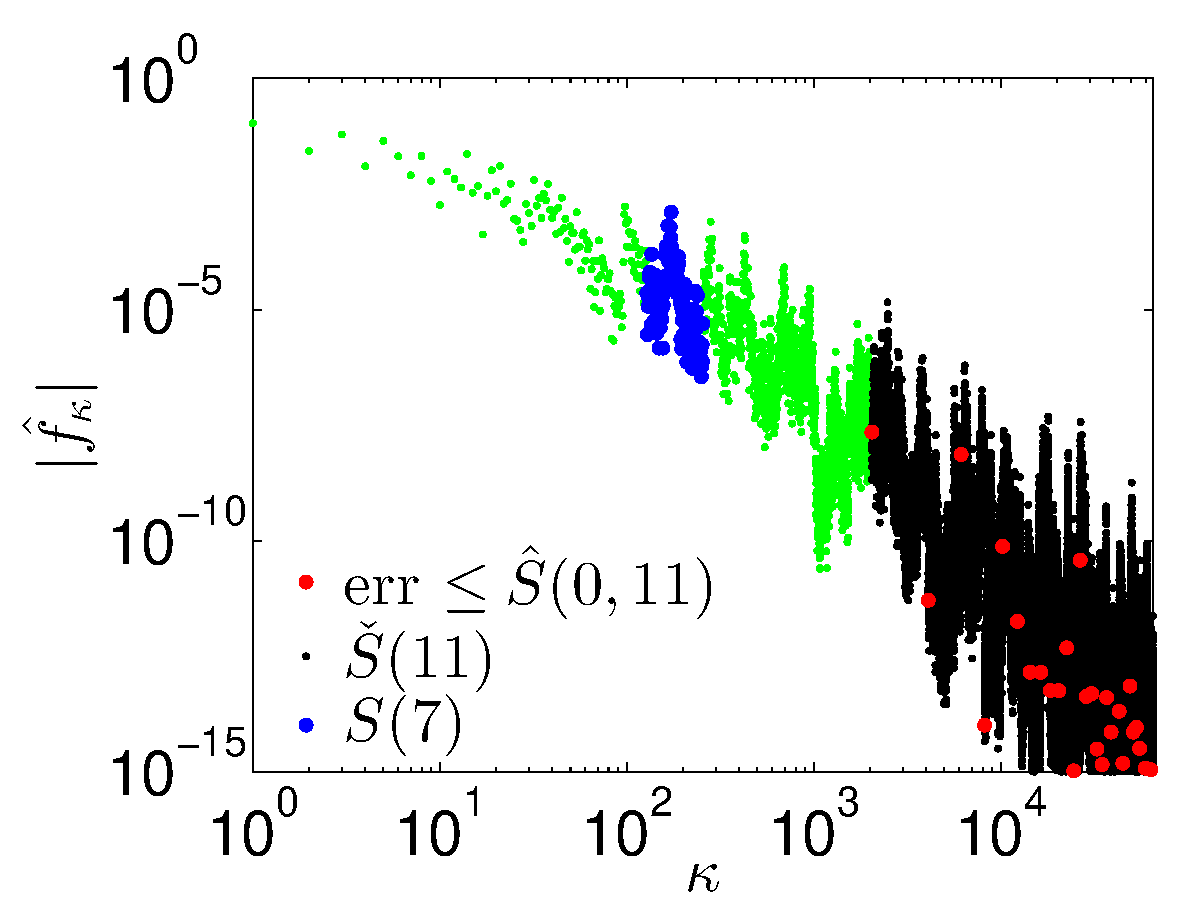
\includegraphics[width=5.6cm]{ProgramsImages/PlotFWTCoefUse128.eps} \quad
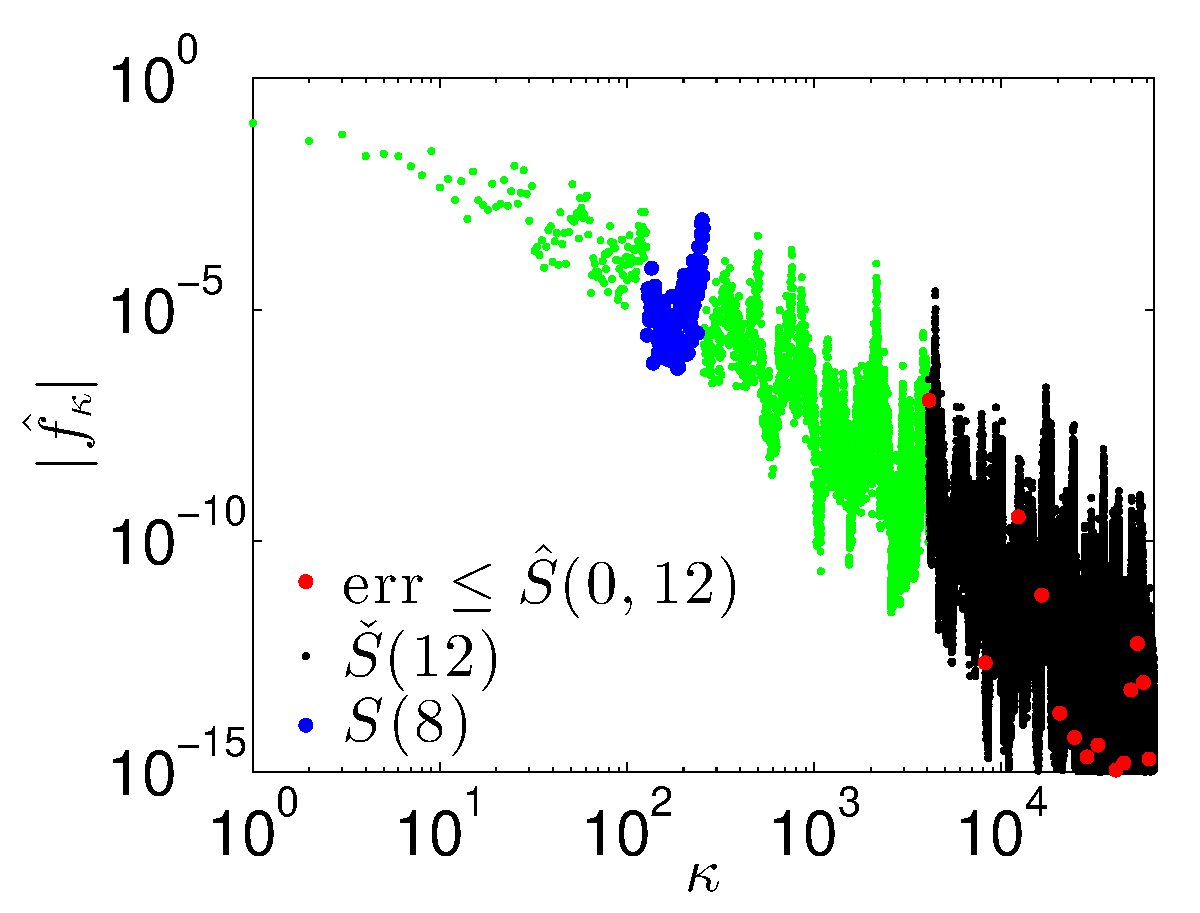
\includegraphics[width=5.6cm]{ProgramsImages/PlotFWTCoefUse256.eps} \quad
\end{center}
\vspace{-3ex}
Make \alert{cone} assumptions on how the $\hf_{\kappa}$ decay.  There exist non-increasing $\homega$ and $\wcomega$ such that for all $0 \le \ell \le m$
\vspace{-1ex}
\begin{gather*}
{\color{red}\hS(\ell,m)}  := \sum_{\kappa=\lfloor 2^{\ell-1} \rfloor}^{2^{\ell}-1} \sum_{\lambda=1}^{\infty} \bigabs{ \hf_{\kappa+\lambda 2^{m}}}, \quad
\wcS(m) :=
\sum_{\kappa=2^{m}}^{\infty} \bigabs{\hf_{\kappa}} \quad
{\color{blue}S(\ell)} :=  \sum_{\kappa=\lfloor 2^{\ell-1} \rfloor}^{2^{\ell}-1} \bigabs{\hf_{\kappa}}\\
{\color{red}\hS(\ell,m)} \le \homega(m-\ell) \wcS(m) \quad \forall \ell, \qquad
\wcS(m) \le \wcomega(m-\ell) {\color{blue}S(\ell)} \quad \forall \ell_* \le \ell.
\end{gather*}
\end{frame}

\begin{frame}\frametitle{Error Bound in Terms of Discrete Fourier-Walsh Coeff.}
Cone conditions:
\vspace{-1ex}
\begin{gather*}
{\color{red}\hS(\ell,m)}  := \sum_{\kappa=\lfloor 2^{\ell-1} \rfloor}^{2^{\ell}-1} \sum_{\lambda=1}^{\infty} \bigabs{ \hf_{\kappa+\lambda 2^{m}}}, \quad
\wcS(m) :=
\sum_{\kappa=2^{m}}^{\infty} \bigabs{\hf_{\kappa}} \quad
{\color{blue}S(\ell)} :=  \sum_{\kappa=\lfloor 2^{\ell-1} \rfloor}^{2^{\ell}-1} \bigabs{\hf_{\kappa}}\\
{\color{red}\hS(\ell,m)} \le \homega(m-\ell) \wcS(m) \quad \forall \ell, \qquad
\wcS(m) \le \wcomega(m-\ell) {\color{blue}S(\ell)} \quad \forall \ell_* \le \ell.
\end{gather*}
Then we can bound the error as follows:
\begin{align*}
\alert{\err(f,2^m, \{\vz_i\})} & = \Biggabs{\sum_{\lambda=1}^{\infty} \hf_{\lambda 2^{m}}} \le \sum_{\lambda=1}^{\infty} \bigabs{\hf_{\lambda 2^{m}}}
= \alert{\hS(0,m)}\\
& \le \homega(m) \wcS(m) \le \homega(m) \wcomega(m-\ell) {\color{blue}S(\ell)} \\
& \le \frac{\homega(m) \wcomega(m-\ell) {\color{blue}\tS(\ell,m)}}{1 - \homega(m-\ell) \wcomega(m-\ell)}
\end{align*}
where
\[
{\color{blue}\tS(\ell,m)} :=\sum_{\kappa=\lfloor 2^{\ell-1} \rfloor}^{2^{\ell}-1} \bigabs{\tf_{m,\kappa}}, \qquad \tf_{m,\kappa}:= \frac{1}{2^m} \sum_{i=0}^{2^m-1} (-1)^{\ip{\tvk(\kappa)}{\vz_i}} f(\vz_i)
\]
\end{frame}

\begin{frame}\frametitle{Guaranteed, Adaptive, Automatic, Sobol' Cubature}
Given an \alert{error tolerance} $\varepsilon>0$ and an integrand $f$, fix the lag $r \in \naturals$ and let
\[
\fC=\frac{\wcomega(r)}{1 - \homega(r) \wcomega(r)}, \qquad m=r+\ell_*.
\]
\begin{description}
\item[Step 1.]  Compute the sum of the (data-based) {\color{blue}discrete Fourier-Walsh coefficients $\tS(m-r,m)$}.
\item[Step 2.] If the \alert{error tolerance} is satisfied,
\[
\fC \homega(m) {\color{blue}\tS(m-r,m)} \le \varepsilon,
\]
then return the Sobol' cubature answer.

\item[Step 3.]  Otherwise, increase $m$ by one, and return to Step 1.

\end{description}

\alert{Theorem.} $\displaystyle \biggabs{\int_{\cube} f(\vx) \, \dif \vx - \frac{1}{2^m} \sum_{i=1}^m f(\vz_i)} \le \varepsilon$ if $f$ satisfies the \alert{cone} conditions on its Fourier-Walsh coefficients.

\end{frame}

\section{Numerical Examples}
\begin{frame}\frametitle{An Example}

\end{frame}

\section{Discussion}
\begin{frame} \frametitle{Guaranteed Automatic Integration Library (GAIL) \url{http://code.google.com/p/gail/}}

\begin{itemize}

\item Version 1.3 (February 14, 2014) \cite{ChoEtal14a} includes \texttt{integral\_g.m}, \texttt{meanMC\_g.m}, \texttt{cubMC\_g.m}, and \texttt{funappx\_g.m}

\item Version 2.0 (exp.\ September 2014) will hopefully include some of the following:
\begin{itemize}
\item quasi-Monte Carlo
\item multi-level Monte Carlo
\item multivariate function approximation
\item relative error criterion

\item higher order methods

\item local adaption

\end{itemize}

\item Theory developed in \ocite{HicEtal14a} and \ocite{HicEtal14b}.  Should be applicable to other problems where
\[
\text{solution}(cf)=\abs{c}\text{solution}(f).
\]

\end{itemize}
\end{frame}

\frame[allowframebreaks]{\frametitle{References}
\bibliography{FJH22,FJHown22}
}

\end{document}



\begin{frame}\frametitle{Error Bound in Terms of {\it True} Fourier-Walsh Coefficients}
Assume $f$ lies in a \alert{cone} defined in terms of how the Fourier-Walsh coefficients decay. There exist non-increasing $\homega$ and $\wcomega$ such that for all $0 \le \ell \le m$
\begin{gather*}
\hS(\ell,m)  := \sum_{\kappa=\lfloor 2^{\ell-1} \rfloor}^{2^{\ell}-1} \sum_{\lambda=1}^{\infty} \bigabs{ \hf_{\kappa+\lambda 2^{m}}}, \quad
\wcS(m) :=
\sum_{\kappa=2^{m}}^{\infty} \bigabs{\hf_{\kappa}} \quad
S(\ell) :=  \sum_{\kappa=\lfloor 2^{\ell-1} \rfloor}^{2^{\ell}-1} \bigabs{\hf_{\kappa}}\\
\hS(\ell,m) \le \homega(m-\ell) \wcS(m) \quad \forall \ell, \qquad
\wcS(m) \le \wcomega(m-\ell) S(\ell) \quad \forall \ell_* \le \ell.
\end{gather*}
Then we can bound the error as follows:
\begin{equation*}
\alert{\err(f,2^m, \{\vz_i\})} \le \sum_{\lambda=1}^{\infty} \bigabs{\hf_{\lambda 2^{m}}}
= \hS(0,m) \le \homega(m) \wcS(m) \le \homega(m) \wcomega(m-\ell) \alert{S(\ell)}.
\end{equation*}
Since we cannot compute $S(\ell)$ from data, we need to bound it in terms of \alert{discrete Fourier-Walsh coefficients}.
\begin{equation*}
\tf_{m,\kappa} := \frac{1}{2^m} \sum_{i=0}^{2^m-1} (-1)^{\ip{\tvk(\kappa)}{\vz_i}} f(\vz_i) = \hf_{\kappa} + \underbrace{\sum_{\lambda=1}^{\infty} \hf_{\kappa+\lambda 2^{m}}}_{\text{aliasing}}.
\label{tfassumc}
\end{equation*}

\end{frame}



\begin{frame}\frametitle{Error Bound in Terms of Discrete Fourier-Walsh Coeff.}
The sum of the true Fourier coefficients can be bounded above in terms of a sum of the discrete Fourier coefficients:
\begin{align*}
S(\ell) &= \sum_{\kappa=\lfloor 2^{\ell-1} \rfloor}^{2^{\ell}-1} \bigabs{\hf_{\kappa}} = \sum_{\kappa=\lfloor 2^{\ell-1} \rfloor}^{2^{\ell}-1} \abs{\tf_{m,\kappa} - \sum_{\lambda=1}^{\infty} \hf_{\kappa+\lambda 2^{m}}} \\
& \le \underbrace{\sum_{\kappa=\lfloor 2^{\ell-1} \rfloor}^{2^{\ell}-1} \bigl \lvert \tf_{m,\kappa} \bigr\rvert}_{\tS(\ell,m)} + \underbrace{\sum_{\kappa=\lfloor 2^{\ell-1} \rfloor}^{2^{\ell}-1} \sum_{\lambda=1}^{\infty} \bigl \lvert \hf_{\kappa+\lambda 2^{m}}\bigr\rvert}_{\hS(\ell,m)} \\
&\le \tS(\ell,m) + \homega(m-\ell) \wcomega(m-\ell) S(\ell) \\
S(\ell) & \le \frac{\tS(\ell,m)}{1 - \homega(m-\ell) \wcomega(m-\ell)} \qquad \text{provided that } \homega(m-\ell) \wcomega(m-\ell) < 1.
\end{align*}
\begin{equation*}
\alert{\err(f,2^m, \{\vz_i\})} \le \homega(m) \wcomega(m-\ell) S(\ell) \le \frac{\homega(m) \wcomega(m-\ell) \alert{\tS(\ell,m)}}{1 - \homega(m-\ell) \wcomega(m-\ell)} .
\end{equation*}

\end{frame}

=======
%MCQMC, April 6-11, 2014
\documentclass[10pt,compress]{beamer} %slides and notes
\usepackage{amsmath,datetime,xmpmulti,mathtools,bbm,array,booktabs,alltt,xspace,mathabx,tikz,pifont,graphicx}
%\usepackage[autolinebreaks]{mcodefred}
\usepackage[author-year]{amsrefs}
\usetikzlibrary{arrows}
\usetheme{FredIIT}

\setlength{\parskip}{2ex}
\setlength{\arraycolsep}{0.5ex}

%\logo{\includegraphics[width=0.5cm]{IIT_mark_1c_red.eps}}
\logo{\includegraphics[width=0.5cm]{MengerIITRedGray.pdf}}

\title[Error Estimation for Sobol' Cubature]{Reliable Error Estimation for Cubature Using \\ Sobol' Sequences}
\author[hickernell@iit.edu]{Fred J. Hickernell \vspace{-4ex}}
\institute{\small{Department of Applied Mathematics,  Illinois Institute of Technology \\
\url{hickernell@iit.edu} \quad
\url{www.iit.edu/~hickernell}\\[2ex]
\emph{In honor of Ilya M. Sobol'}\\[2ex]
Joint work with Llu\'is Antoni Jim\'enez Rugama\\
speaking tomorrow, 11:15 am on lattice rules\\[2ex]
Supported by NSF-DMS-1115392}}
\date[MCQMC 2014]{April 10, 2014}

%The error in approximating the multidimensional integral $\int_{[0,1)^d} f(\boldsymbol{x}) \, {\rm d} \boldsymbol{x}$ by the sample average $n^{-1} \sum_{i=0}^{n-1} f(\boldsymbol{x}_i)$ depends on both the sampling scheme, $\{\boldsymbol{x}_0, \boldsymbol{x}_1, \ldots \}$, and the integrand, $f$.  Quasi-Monte Carlo methods, such as Sobol' sampling, are often substantially more efficient than IID sampling for evaluating multidimensional integrals.  A reliable data-based error bound is needed so that one can automatically determine the appropriate sample size, $n$, to satisfy a user-supplied error tolerance $\varepsilon$.  Koksma-Hlawka error bounds require a priori knowledge of the variation of $f$.  Quasi-standard error \cite{Hal05a} can be fooled by functions, $f$, that are not particularly strange \cite{Owe06a}.  The same is true for internal replications.  Error estimates based on $M$ IID replications of $n$ randomized Sobol' sample points do not inform how much larger $n$ should be to satisfy the error tolerance.

%This talk presents a new method for bounding the error of quasi-Monte Carlo cubature based on Sobol' sampling.  The method depends on the discrete Walsh transform of the sampled function values and assumptions on the decay rate of the Walsh series for $f$.  The error bound can be conveniently updated as $n$ is doubled until the error tolerance is satisfied. Like the recently proposed automatic cubature method based on IID sampling \cite{HicEtal14a}, the method proposed here is guaranteed for a cone of integrands. 


\input FJHDef.tex

\newcommand{\tol}{\text{tol}}
\DeclareMathOperator{\cubMC}{cubMC}
\DeclareMathOperator{\qse}{qse}
\DeclareMathOperator{\integ}{int}
\DeclareMathOperator{\trap}{trap}
\DeclareMathOperator{\size}{size}
\DeclareMathOperator{\app}{id}
\DeclareMathOperator{\err}{err}
\DeclareMathOperator{\walsh}{walsh}
\newcommand{\happ}{\widehat{\app}}
\newcommand{\hinteg}{\widehat{\integ}}
\newcommand{\cube}{[0,1)^d}
\newcommand{\desall}{\{\vz_i\}}
\newcommand{\desn}{\{\vz_i\}_{i=0}^{n-1}}
\def\newblock{\hskip .11em plus .33em minus .07em}
\newcommand{\wcS}{\widecheck{S}}
\newcommand{\wcomega}{\widecheck{\omega}}



\begin{document}
\tikzstyle{every picture}+=[remember picture]

\frame{\titlepage}

\section{Problem}
\begin{frame}\frametitle{Automatic, Adaptive Quasi-Monte Carlo Cubature}
\vspace{-3ex}
\begin{tabular}{>{\flushleft}m{5.5cm}@{\qquad}>{\flushleft}m{5.5cm}}
\begin{multline*}
\uncover<3->{\err(f,n,\desall) := \\
\Biggl \lvert}\int_{\cube} f(\vx) \, \dif \vx 
\only<1>{= ?}
\uncover<2->{\only<2>{\approx}\only<3->{-} \frac 1 n \sum_{i=0}^{n-1} f(\vz_i)}
\uncover<3->{\Biggr \rvert \\ 
\le \underbrace{D(n,\desall)}_{\text{quality of } \desall} \ \underbrace{V(f)}_{\text{roughness of } f }}
\\[2ex]
\end{multline*} 
\uncover<4->{How to \alert{automatically} and \alert{adaptively} choose $n$ to ensure 
\[
\err(f,n,\desall) \le \varepsilon?
\]
(nonlinear algorithm, \\
non-convex set of integrands)}
&
option pricing, statistical physics, photon transport, \ldots \\[1ex]
\uncover<2->{$\{\vz_i\}$ chosen IID $\cu\cube$, \cite{Ric51}, \cite{Kor59}, \cite{Hal60}, \alert{\cite{Sob67}}, \cite{Fau82}, \ldots} \\[1ex]
\uncover<3->{better points, tractability, multi-level \cite{Hla61}, \cite{Nie92}, \cite{SloJoe94}, \cite{Hic97a}, \cite{DicPil10a}, \cite{NovWoz10a}, \cite{DicEtal14a} \cite{Gil14a}, \ldots } \\[1ex]
\uncover<4->{guaranteed, automatic, adaptive Monte Carlo \cite{HicEtal14a}, trapezoidal rule \cite{HicEtal14b}, GAIL \cite{ChoEtal14a}}
\tabularnewline
\end{tabular}
\end{frame}

\begin{frame}\frametitle{Sobol' Points}
Let $\oplus$ denote binary \alert{digit by digit} addition modulo 2:
\begin{equation*}
\frac 18 \oplus \frac 58 = {}_20.001 \oplus {}_20.101 = \oplus {}_20.100 = \frac 12, \qquad
1 \oplus 5 = 001_2 \oplus 101_2 = 100_2 = 4
\end{equation*}
\begin{tabular}{m{5.7cm}>{\centering}m{5.7cm}}
Sobol' points $\desall$ satisfy
\begin{equation*}
\vz_0=\vzero, \quad \vz_i \oplus \vz_\ell = \vz_{i\oplus \ell} \quad \forall i,\ell \in \natzero
\end{equation*}
$\begin{aligned}
\vz_1\oplus\vz_5 &= ({}_20.100, {}_20.100) \\
& \qquad \qquad \oplus ({}_20.101, {}_20.001) \\
&= ({}_20.001, {}_20.101) \\
& = \vz_4=\vz_{1\oplus 5}
\end{aligned}$
&
\includegraphics[width=5.7cm]{ProgramsImages/scrsob1024pts.eps}
\end{tabular}
\end{frame}

\begin{frame}\frametitle{Walsh Functions}
\vspace{-2ex}
The base-$2$ Walsh function, \alert{$\walsh(\cdot,\cdot) : (\vk,\vx) \mapsto (-1)^{\ip{\vk}{\vx}}$}, is defined in terms of the a bilinear function $\ip{\cdot}{\cdot}: \natzero^d \times \cube \to \{0,1\}$:
\vspace{-2ex}
\begin{gather*}
\ip{\vk}{\vx} = \ip{(k_1, \ldots, k_d) }{(x_1, \ldots, x_d)} := \sum_{j=1}^d \ip{k_j}{x_j} \bmod 2 \\
\ip{k_j}{x_j} = \ip{(\cdots k_{j1} k_{j0})_2}{{}_20.x_{j1} x_{j2} \cdots} := k_{j0} x_{j1} + k_{j1} x_{j2} + \cdots \bmod 2
\end{gather*}
\begin{center}
\includegraphics[width=3cm]{ProgramsImages/walshk0fun.eps} \qquad
\includegraphics[width=3cm]{ProgramsImages/walshk1fun.eps} \qquad
\includegraphics[width=3cm]{ProgramsImages/walshk2fun.eps} \\
\includegraphics[width=3cm]{ProgramsImages/walshk3fun.eps} \qquad
\includegraphics[width=3cm]{ProgramsImages/walshk4fun.eps} \qquad
\includegraphics[width=3cm]{ProgramsImages/walshk5fun.eps} 
\end{center}
\end{frame}

\begin{frame}\frametitle{Sobol' Cubature Error via Fourier-Walsh Expansions}
The Fourier-Walsh expansion of an integrand is given by 
\[
f(\vx) = \sum_{\vk \in \natzero^d} (-1)^{\ip{\vk}{\vx}} \hf(\vk) , \qquad \text{where } \hf(\vk) := \int_{\cube} f(\vx)(-1)^{\ip{\vk}{\vx}} \, \dif \vx.
\]
Sobol' points integrate most Walsh functions perfectly, but some terribly:
\[
\frac 1 {2^m} \sum_{i=0}^{2^m-1} (-1)^{\ip{\vk}{\vz_i}} =
\begin{cases} 1, & \vk \in \cp^{\perp}_m := \{ \vk \in \natzero^d : \ip{\vk}{\vz_i}=0, \ i=0, \ldots 2^{m}-1\}, \\
0 & \vk \notin \cp^{\perp}_m
\end{cases}
\]
So Sobol' cubature error depends on the sizes of the Fourier-Walsh coefficients for $\vk$ in the \alert{dual Sobol' set} $\cp^{\perp}_m$:
\[
\err(f,2^m,\desall) := 
\Biggabs{\int_{\cube} f(\vx) \, \dif \vx -  \frac 1 {2^m} \sum_{i=0}^{2^m-1} f(\vz_i)} = 
\Biggabs{\sum_{\vk \in \cp^{\perp}_m\setminus\{\vzero\}} \hf(\vk)}
\]
\alert{How do we reliably bound this error based on the $f(\vz_i)$?}
\end{frame}

\section{Error Bounds Based on Cones}
\begin{frame}\frametitle{Wavenumber Map}
Define a bijective  mapping $\tvk:\natzero \to \natzero^d$ such that for all $m,\lambda \in \natzero$ and $\kappa=0, \ldots, 2^m-1$,
\begin{gather*}
\tvk(0) = \vzero, \qquad \tvk(\kappa+\lambda 2^m)=\tvk(\kappa) \oplus \vl \text{ for some }\vl \in \cp_m^{\perp}, \\
\text{e.g., } \tvk(29) = \tvk(5) \oplus \vl \text{ for some }\vl \in \cp_3^{\perp}, \text{ but not for some }\vl \in \cp_4^{\perp}
\end{gather*}
One can express the Fourier-Walsh expansion for the integrand and the error as 
\begin{equation*}
f(\vx) = \sum_{\kappa=0}^{\infty} (-1)^{\ip{\tvk(\kappa)}{\vx}} \hf_{\kappa}, \qquad
\hf_{\kappa}:=\hf(\tvk(\kappa)), \qquad 
\err(f,2^m,\desall) = \Biggabs{\sum_{\lambda=1}^{\infty} \hf_{\lambda 2^m}}
\end{equation*}
\alert{Large $\kappa$ implies typically smaller $\hf_{\kappa}$} in a way that is made explicit on the next slide.
Moreover, the \alert{discrete} Fourier-Walsh coefficients are \alert{aliased} as follows:
\begin{gather*}
\tf_{m,\kappa}:= \frac{1}{2^m} \sum_{i=0}^{2^m-1} (-1)^{\ip{\tvk(\kappa)}{\vz_i}} f(\vz_i) \qquad 
\tf_{m,\kappa+\lambda 2^m} = \tf_{m,\kappa}, \\ 
\text{e.g., } \tf_{3,29} = \tf_{3,5}, \text{ but generally } \hf_{29} \ne \hf_{5} \text{ and } \tf_{4,29} \ne \tf_{4,5}
\end{gather*}

\end{frame}

\begin{frame}\frametitle{Cone Assumptions on Decay of Fourier Walsh Coefficients}
\begin{center}
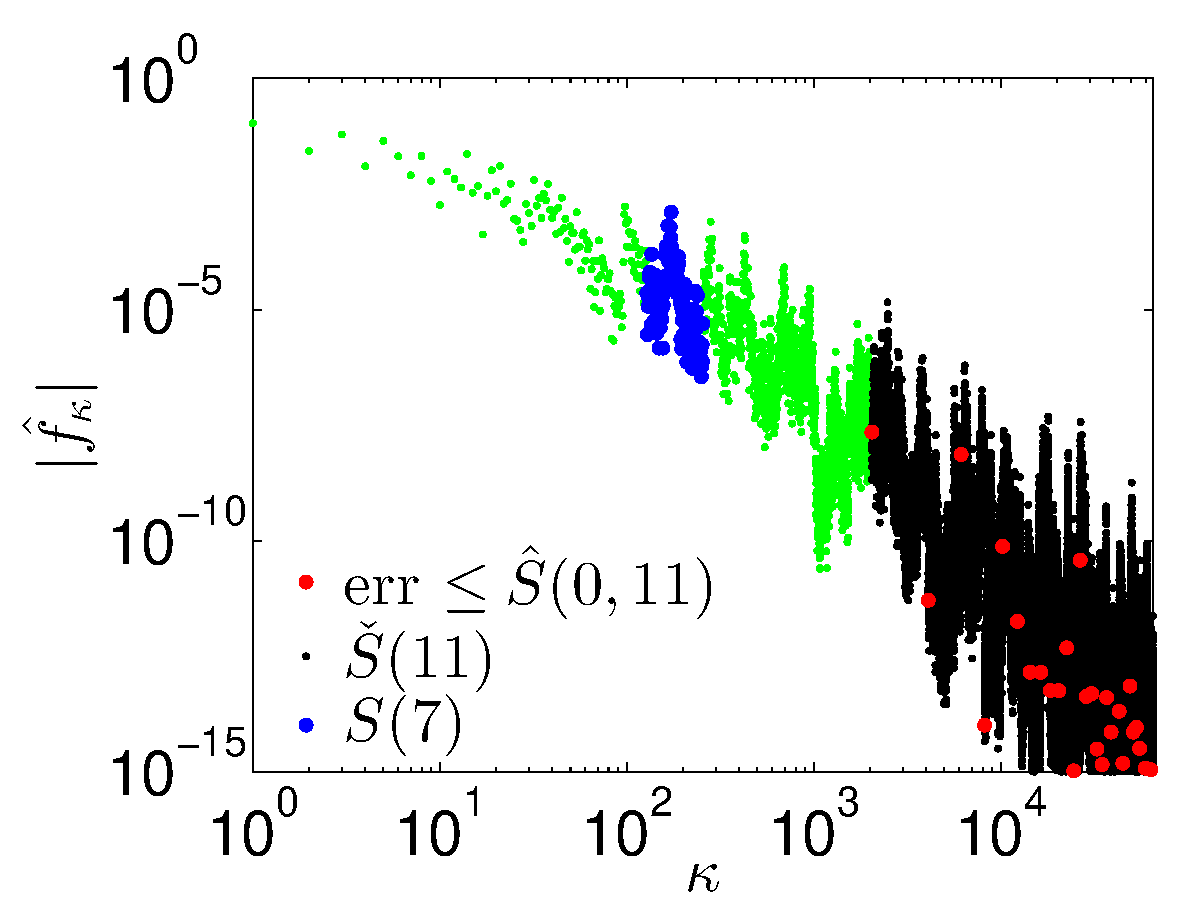
\includegraphics[width=5.6cm]{ProgramsImages/PlotFWTCoefUse128.eps} \quad
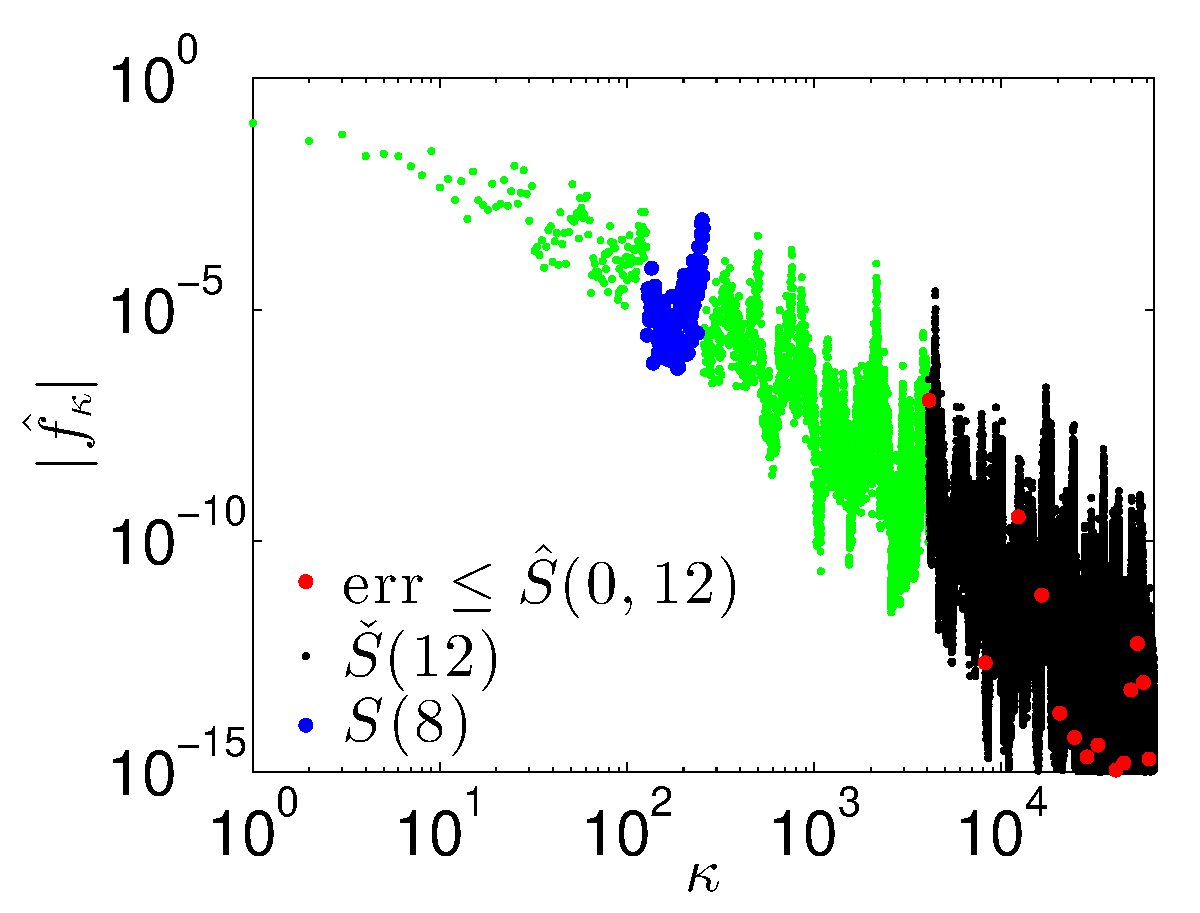
\includegraphics[width=5.6cm]{ProgramsImages/PlotFWTCoefUse256.eps} \quad
\end{center}
\vspace{-3ex}
Make \alert{cone} assumptions on how the $\hf_{\kappa}$ decay.  There exist non-increasing $\homega$ and $\wcomega$ such that for all $0 \le \ell \le m$
\vspace{-1ex}
\begin{gather*}
{\color{red}\hS(\ell,m)}  := \sum_{\kappa=\lfloor 2^{\ell-1} \rfloor}^{2^{\ell}-1} \sum_{\lambda=1}^{\infty} \bigabs{ \hf_{\kappa+\lambda 2^{m}}}, \quad
\wcS(m) :=
\sum_{\kappa=2^{m}}^{\infty} \bigabs{\hf_{\kappa}} \quad 
{\color{blue}S(\ell)} :=  \sum_{\kappa=\lfloor 2^{\ell-1} \rfloor}^{2^{\ell}-1} \bigabs{\hf_{\kappa}}\\
{\color{red}\hS(\ell,m)} \le \homega(m-\ell) \wcS(m), \qquad 
\wcS(m) \le \wcomega(\ell) {\color{blue}S(m-\ell)} \quad \forall m \ge \ell+\ell_*.
\end{gather*}
\end{frame}

\begin{frame}[label=errbdDFWT]\frametitle{Error Bound in Terms of Discrete Fourier-Walsh Coeff.}
Cone conditions:
\vspace{-1ex}
\begin{gather*}
{\color{red}\hS(\ell,m)}  := \sum_{\kappa=\lfloor 2^{\ell-1} \rfloor}^{2^{\ell}-1} \sum_{\lambda=1}^{\infty} \bigabs{ \hf_{\kappa+\lambda 2^{m}}}, \quad
\wcS(m) :=
\sum_{\kappa=2^{m}}^{\infty} \bigabs{\hf_{\kappa}} \quad 
{\color{blue}S(\ell)} :=  \sum_{\kappa=\lfloor 2^{\ell-1} \rfloor}^{2^{\ell}-1} \bigabs{\hf_{\kappa}}\\
{\color{red}\hS(\ell,m)} \le \homega(m-\ell) \wcS(m) \quad \forall \ell, \qquad 
\wcS(m) \le \wcomega(\ell) {\color{blue}S(m-\ell)} \quad \forall m \ge \ell+\ell_*.
\end{gather*}
Then we can bound the error as follows:
\begin{align*}
\alert{\err(f,2^m, \{\vz_i\})} & = \Biggabs{\sum_{\lambda=1}^{\infty} \hf_{\lambda 2^{m}}} \le \sum_{\lambda=1}^{\infty} \bigabs{\hf_{\lambda 2^{m}}} 
= \alert{\hS(0,m)}\\
& \le \homega(m) \wcS(m) \le \homega(m) \wcomega(\ell) {\color{blue}S(m-\ell)} \\
& \le \frac{\homega(m) \wcomega(\ell) {\color{blue}\tS(m-\ell,m)}}{1 - \homega(\ell) \wcomega(\ell)} \quad \beamerbutton{\hyperlink{SboundbytS}{proof}}
\end{align*}
where 
\[
{\color{blue}\tS(\ell,m)} :=\sum_{\kappa=\lfloor 2^{\ell-1} \rfloor}^{2^{\ell}-1} \bigabs{\tf_{m,\kappa}}, \qquad \tf_{m,\kappa}:= \frac{1}{2^m} \sum_{i=0}^{2^m-1} (-1)^{\ip{\tvk(\kappa)}{\vz_i}} f(\vz_i)
\]
\end{frame}

\begin{frame}[label=algothm]\frametitle{\texttt{cubSobol\_g}---Guaranteed, Adaptive, Sobol' Cubature}
\vspace{-2ex}
Given an \alert{error tolerance} $\varepsilon>0$ and an integrand $f$, fix the lag $\ell \in \naturals$ and let
\[
\fC=\frac{\wcomega(\ell)}{1 - \homega(\ell) \wcomega(\ell)}, \qquad m=\ell+\ell_*.
\]
\vspace{-4ex}
\begin{description}
\item[Step 1.]  Compute the sum of the (data-based) {\color{blue}discrete Fourier-Walsh coefficients $\tS(m-\ell,m)$}.  
\item[Step 2.] If the \alert{error tolerance} is satisfied, i.e.,
\[
\fC \homega(m) {\color{blue}\tS(m-\ell,m)} \le \varepsilon,
\]
then return the Sobol' cubature answer.

\item[Step 3.]  Otherwise, increase $m$ by one, and return to Step 1.

\end{description}

\alert{Theorem.} If $f$ satisfies the \alert{cone} conditions on its Fourier-Walsh coefficients, then 
\[
\biggabs{\int_{\cube} f(\vx) \, \dif \vx - \frac{1}{2^m} \sum_{i=0}^{2^m-1} f(\vz_i)} \le \varepsilon 
\]
at a computational cost of $\Order([m + \$(f)]2^m )$, where $\$(f)$ is the cost of a function evaluation and $m \le \min \{m' : \fC \homega(m') [1+ \homega(\ell) \wcomega(\ell)] {\color{blue}S(m'-\ell)} \le \varepsilon \}$ \beamerbutton{\hyperlink{tSboundbyS}{proof}}.

\end{frame}

\section{Numerical Examples}
\begin{frame}\frametitle{Asian Geometric Mean Call Option}
\begin{gather*}
S(0)=K=100, \quad T=1, \quad r=0.03, \quad \text{volatility} \sim \cu[0.1,0.7],\\
 d = \text{\# time steps} \sim \cu \{1,2,4,8,16,32,64\}
\end{gather*}
\begin{tabular}{>{\centering}m{5.7cm}>{\centering}m{5.7cm}}
IID, \texttt{cubMC\_g} & Sobol', \texttt{cubSobol\_g} \tabularnewline
\includegraphics[width=5.7cm]{ProgramsImages/geomeaniidErrTime.eps} & 
\includegraphics[width=5.7cm]{ProgramsImages/geomeancubSobolErrTime.eps}
\end{tabular}
\end{frame}

\begin{frame}\frametitle{Genz and Keister Examples}
These examples come from \ocite{Gen87} and \ocite{Kei96}
\begin{center}
\begin{tabular}{>{\centering}m{7.5cm}>{\raggedright}m{3.5cm}}
\texttt{cubSobol\_g} \tabularnewline
\includegraphics[width=7.5cm]{ProgramsImages/GenzcubSobolErrTime.eps} &
\alert{$\bullet$} within budget \newline
{\color{brown}{$\bullet$}} exceeded budget
\end{tabular}
\end{center}
\end{frame}

\section{Discussion}
\begin{frame} \frametitle{What's Missing for \texttt{cubSobol\_g}?}

\begin{itemize}

\item Connections between our cone conditions and \alert{familiar spaces} of integrands, such as Korobov spaces

\item Lower bound on the \alert{computational complexity}

\item \alert{Relative} error criterion

\item Justification for our heuristic determination of the map $\kappa$

\end{itemize}

\end{frame}

\begin{frame}\frametitle{Why Not Replications to Estimate Error?}
\vspace{-3ex}
\[
\Biggabs{\int_{\cube} f(\vx) \, \dif \vx 
- \hmu_n} \le \fC \sqrt{\frac{1}{R-1}\sum_{r=1}^R (Y_{r} - \hmu_n)^2},  \qquad \hmu_n:=\frac 1 R \sum_{r=1}^{R} Y_r
\]
\begin{description}

\item[IID Replications] $\displaystyle Y_{r}=\frac{R}{n}\sum_{i=0}^{n/R-1} f(\vz_i^{(r)})$, where $\{\vz_i^{(r)}\}$ are independent randomizations. 

\item[Internal Replications] $\displaystyle Y_{r}=\frac{R}{n}\sum_{i=(r-1)n/R}^{rn/R-1} f(\vz_i)$. 

\end{description}
Want $R$ small to take advantage of Sobol' point evenness, but need $R$ large to ensure that sample variance of $Y_r$ represents error \cite{Den13a,HicEtal14a}.  

\end{frame}


\begin{frame} \frametitle{Guaranteed Automatic Integration Library (GAIL) \url{http://code.google.com/p/gail/}}

\begin{itemize}

\item Version 1.3 (February 14, 2014) \cite{ChoEtal14a} includes \texttt{integral\_g.m}, \texttt{meanMC\_g.m}, \texttt{cubMC\_g.m}, and \texttt{funappx\_g.m} 

\item Version 2.0 (exp.\ September 2014) will hopefully include some of the following:
\begin{itemize} 
\item quasi-Monte Carlo---\texttt{cubSobol\_g.m}, \texttt{cubLattice\_g.m}
\item Monte Carlo for Bernoulli---\texttt{meanBernoulli\_g.m}
\item multi-level Monte Carlo---\texttt{meanMLMC\_g.m}
\item multivariate function approximation
\item relative error criterion

\item higher order methods (for one dimensional problems)

\item local adaption (for one dimensional problems)

\end{itemize}

\item Theory developed in \ocite{HicEtal14a} and \ocite{HicEtal14b}.  Should apply to other problems where 
\[
\text{solution}(cf)=\abs{c}\text{solution}(f).
\]

\end{itemize}
\end{frame}

\frame[allowframebreaks]{\frametitle{References}
\bibliography{FJH22,FJHown22}
}

\begin{frame}[label=SboundbytS]\frametitle{Bounding {\color{blue}$S(\ell)$} in Terms of {\color{blue}$\tS(\ell,m)$} }
\begin{align*}
{\color{blue}S(\ell)} &= \sum_{\kappa=\lfloor 2^{\ell-1} \rfloor}^{2^{\ell}-1} \bigabs{\hf_{\kappa}} = \sum_{\kappa=\lfloor 2^{\ell-1} \rfloor}^{2^{\ell}-1} \abs{\tf_{m,\kappa} - \sum_{\lambda=1}^{\infty} \hf_{\kappa+\lambda 2^{m}}} \\
& \le \underbrace{\sum_{\kappa=\lfloor 2^{\ell-1} \rfloor}^{2^{\ell}-1} \bigl \lvert \tf_{m,\kappa} \bigr\rvert}_{{\color{blue}\tS(\ell,m)}} + \underbrace{\sum_{\kappa=\lfloor 2^{\ell-1} \rfloor}^{2^{\ell}-1} \sum_{\lambda=1}^{\infty} \bigl \lvert \hf_{\kappa+\lambda 2^{m}}\bigr\rvert}_{\hS(\ell,m)} \\
&\le {\color{blue}\tS(\ell,m)} + \homega(m-\ell) \wcomega(m-\ell) {\color{blue}{S(\ell)}}  \\
{\color{blue}S(\ell)} & \le \frac{{\color{blue}\tS(\ell,m)}}{1 - \homega(m-\ell) \wcomega(m-\ell)} \qquad \text{provided that } \homega(m-\ell) \wcomega(m-\ell) < 1
\end{align*}
 \hfill \hfill \beamerreturnbutton{\hyperlink{errbdDFWT}{back}}
\end{frame}

\begin{frame}[label=tSboundbyS]\frametitle{Bounding {\color{blue}$\tS(\ell,m)$} in Terms of {\color{blue}$S(\ell)$}}
\begin{align*}
{\color{blue}\tS(\ell,m)} &= \sum_{\kappa=\lfloor 2^{\ell-1} \rfloor}^{2^{\ell}-1} \bigabs{\tf_{m,\kappa}} = \sum_{\kappa=\lfloor 2^{\ell-1} \rfloor}^{2^{\ell}-1} \abs{\hf_{\kappa} + \sum_{\lambda=1}^{\infty} \hf_{\kappa+\lambda 2^{m}}} \\
& \le \underbrace{\sum_{\kappa=\lfloor 2^{\ell-1} \rfloor}^{2^{\ell}-1} \bigabs{ \hf_{\kappa}}}_{{\color{blue}\hS(\ell)}} + \underbrace{\sum_{\kappa=\lfloor 2^{\ell-1} \rfloor}^{2^{\ell}-1} \sum_{\lambda=1}^{\infty} \bigl \lvert \hf_{\kappa+\lambda 2^{m}}\bigr\rvert}_{\hS(\ell,m)} \\
&\le [1 + \homega(m-\ell) \wcomega(m-\ell)] {\color{blue}{S(\ell)}}
\end{align*}
 \hfill \hfill \beamerreturnbutton{\hyperlink{algothm}{back}}
\end{frame}

\end{document}

>>>>>>> d07e907edac143851f64f6a820b0080df3178639
